\documentclass[12pt]{report}

% Packages
% ========
\usepackage[letterpaper, portrait, margin=1in]{geometry}
\usepackage{graphicx}			% So we can load figures with "." in their filename
\usepackage{float}				% So we can use "[H]"
\usepackage[dvipsnames]{xcolor}	% For custom colors
\usepackage{xparse}				% For \DeclareDocumentCommand
\usepackage{caption}			% For \captionof command
\usepackage{mathtools}			% For \DeclarePairedDelimeter
\usepackage{ifthen}				% For \ifthenelse{}{}{}
\usepackage{soul}				% For underlining with \ul
\setuldepth{x}					%	""
\usepackage{multicol}			% For multiple columns via \begin{multicols}{2}
\usepackage[most]{tcolorbox}	% For the tl; dr environment
\usepackage{array}				% For extended column definitions
\usepackage{tabularray}			% For \begin{longtblr} tables that span multiple columns and pages
\usepackage{amssymb}			% For $\checkmark$
\usepackage{etoc}				% For \localtableofcontents


% Bibliography
% ============
\usepackage[american]{babel}
\usepackage{csquotes}
\usepackage[style=ieee, backend=biber]{biblatex}
\usepackage{hyperref}
\hypersetup{colorlinks=true, allcolors=black, urlcolor=blue}
\addbibresource{../sources.bib}

% etoc setup
% ==========

\etocsetstyle{section}{}{}{\etocsavedchaptertocline{\numberline{}\etocname}{\etocpage}}{}
\etocsetstyle{subsection}{}{}{\etocsavedsectiontocline{\numberline{}\etocname}{\etocpage}}{}
\etocsetstyle{subsubsection}{}{}{\etocsavedsubsectiontocline{\numberline{}\etocname}{\etocpage}}{}
\etocsetstyle{paragraph}{}{}{\etocsavedsubsubsectiontocline{\numberline{}\etocname}{\etocpage}}{}
\etocsetstyle{subparagraph}{}{}{\etocsavedparagraphtocline{\numberline{}\etocname}{\etocpage}}{}


% Simple custom commands
% ======================
\makeatletter
\def\maxwidth#1{\ifdim\Gin@nat@width>#1 #1\else\Gin@nat@width\fi} 
\makeatother

\def\todo#1{\selectfont{\color{red}\texttt{\textbf{TODO:} #1}}}

% Sections 'n' such
% =================

\definecolor{chaptColor}{RGB}{0, 83, 161}

\def\chapt#1{
%
	% Default chapter behavior
	\begingroup\color{chaptColor}
	\chapter{#1}
	\endgroup
	
	% Label
	\label{chp:#1}
}

\definecolor{sectColor}{rgb}{0, 0.5, 0.0}
\def\sect#1{\textcolor{sectColor}{\section{#1}}}

\definecolor{subsectColor}{rgb}{0, 0.5, 0.5}
\def\subsect#1{\textcolor{subsectColor}{\subsection{#1}}\noindent}

\definecolor{subsubsectColor}{rgb}{0.747, 0.458, 0}
\def\subsubsect#1{\textcolor{subsubsectColor}{\subsubsection{#1}}}

% TL; DR section
% ==============
\newenvironment{tldr}{\begin{tcolorbox}[colback=gray!20!white,colframe=blue!75!black,title=TL; DR]}{\end{tcolorbox}\vspace*{12pt}}

% Custom math commands
% ====================
\DeclarePairedDelimiter\ceil{\lceil}{\rceil}
\DeclarePairedDelimiter\floor{\lfloor}{\rfloor}

% ======================
% \graphic{filename=...}
% ======================
% Keyword arguments
\makeatletter
\define@key{graphicKeys}{filename}{\def\graphic@filename{#1}}
\define@key{graphicKeys}{scale}{\def\graphic@scale{#1}}
\define@key{graphicKeys}{width}{\def\graphic@width{#1}}
\define@key{graphicKeys}{caption}{\def\graphic@caption{#1}}
\define@key{graphicKeys}{captionType}{\def\graphic@captionType{#1}}
\define@key{graphicKeys}{label}{\def\graphic@label{#1}}

% Kwargs
\DeclareDocumentCommand{\graphic}{m}{

	\begingroup
	
	% Set default kwargs
	\setkeys{graphicKeys}{filename={0}, #1}
	\setkeys{graphicKeys}{scale={0}, #1}
	\setkeys{graphicKeys}{width={0}, #1}
	\setkeys{graphicKeys}{caption={}, #1}
	\setkeys{graphicKeys}{captionType={figure}, #1}
	\setkeys{graphicKeys}{label={}, #1}
	
	% Assign width
	\let\graphicWidth\relax % let \mytmplen to \relax
	\newlength{\graphicWidth}
	\setlength{\graphicWidth}{\columnwidth}
	
	\if \graphic@scale 0
		
		\if \graphic@width 0
			
			\setlength{\graphicWidth}{0.7\columnwidth}
		
		\else
	
			\setlength{\graphicWidth}{\graphic@width}
			
		\fi

	\else
		
		\setlength{\graphicWidth}{\columnwidth * \graphic@scale}

	\fi	
	
	% Do figure
	\begin{minipage}{\columnwidth}
		\vspace*{12pt}
		\begin{center}
		
			\includegraphics[width = \graphicWidth]{\graphic@filename}
			
			\ifthenelse{\equal{\graphic@caption}{}}{}{
				\captionof{\graphic@captionType}{\graphic@caption}
			}
			
			\ifthenelse{\equal{\graphic@label}{}}{
				\label{fig: \graphic@filename}
			}{
				\label{\graphic@label}
			}
		\end{center}
		\vspace*{12pt}
	\end{minipage}
	
	\endgroup
}
\makeatother

% ==============
% Base Pair Page
% ==============
% Keyword arguments
\makeatletter
\define@key{bpPageKeys}{baseFilename}{\def\bpPage@baseFilename{#1}}
\define@key{bpPageKeys}{scale}{\def\bpPage@scale{#1}}
\define@key{bpPageKeys}{width}{\def\bpPage@width{#1}}
\define@key{bpPageKeys}{caption}{\def\bpPage@caption{#1}}
\define@key{bpPageKeys}{captionType}{\def\bpPage@captionType{#1}}
\define@key{bpPageKeys}{label}{\def\bpPage@label{#1}}

% Kwargs
\DeclareDocumentCommand{\BPPage}{m}{

	\begingroup
	
	% Set default kwargs
	\setkeys{bpPageKeys}{baseFilename={0}, #1}
	\setkeys{bpPageKeys}{caption={}, #1}
	\setkeys{bpPageKeys}{label={}, #1}
	
	\newpage

	\begin{center}
		\ul{\mbox{\bpPage@baseFilename{}: 1 Base Pair [min]}}
	\end{center}
	\vspace*{-36pt}
	\begin{minipage}[b]{0.5\textwidth}
		\graphic{filename=\bpPage@baseFilename-overview-1-table, width=\textwidth}
	\end{minipage}
	\begin{minipage}[b]{0.5\textwidth}
		\graphic{filename=\bpPage@baseFilename-overview-1-plot, width=\textwidth}
	\end{minipage}

	\begin{center}
		\ul{\mbox{\bpPage@baseFilename{}: 50 Base Pairs [average]}}
	\end{center}
	\vspace*{-36pt}
	\begin{minipage}[b]{0.5\textwidth}
		\graphic{filename=\bpPage@baseFilename-overview-50-table, width=\textwidth}
	\end{minipage}
	\begin{minipage}[b]{0.5\textwidth}
		\graphic{filename=\bpPage@baseFilename-overview-50-plot, width=\textwidth}
	\end{minipage}
	
	\begin{center}
		\ul{\mbox{\bpPage@baseFilename{}: 100 Base Pairs [max]}}
	\end{center}
	\vspace*{-36pt}
	\begin{minipage}[b]{0.5\textwidth}
		\graphic{filename=\bpPage@baseFilename-overview-100-table, width=\textwidth}
	\end{minipage}
	\begin{minipage}[b]{0.5\textwidth}
		\graphic{filename=\bpPage@baseFilename-overview-100-plot, width=\textwidth}
	\end{minipage}

	\vspace*{-24pt}
	\captionof{figure}{\bpPage@caption}\label{\bpPage@label}	
	
	\endgroup
}
\makeatother



\begin{document}

% ================

\newpage

\graphic{filename=box-art, width=0.9\textwidth}

% ================

\newpage
{\huge{Hardware}}
\graphic{filename=Misc/hardware, caption={Hardware: Wii 25th anniversary dual-disc edition on a Wii U with a small child who was there for 100\% of this run.}}

% ================

\newpage

% Completion overview
\begin{figure}[H]
		\centering
		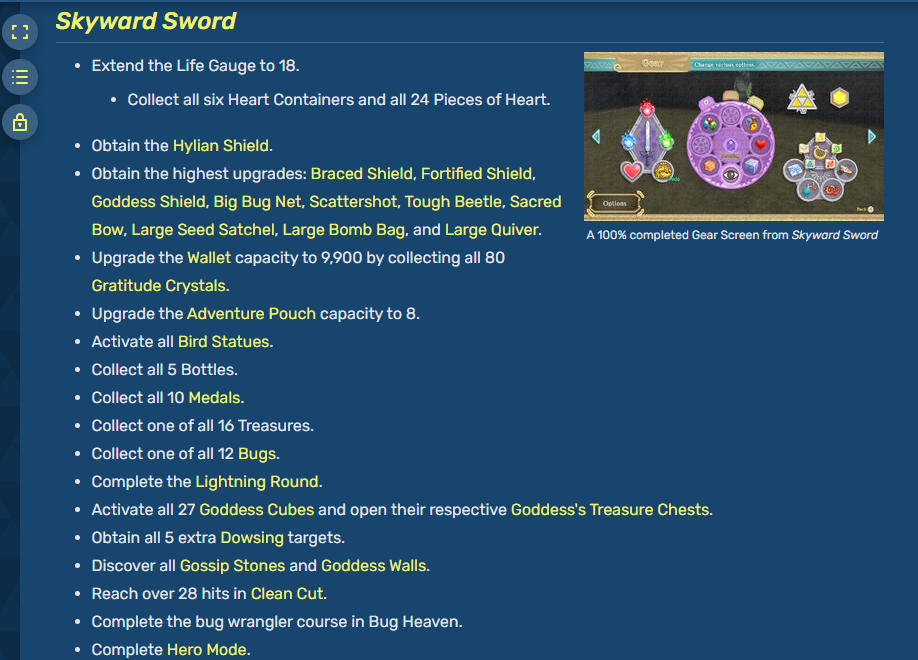
\includegraphics[scale=2]{completion-images/completion}
		\caption{Overview of completion goals.}
	\end{figure}
	
\newpage

% ToC
\etocsettocstyle{}{}
\localtableofcontents

% ================

\newpage
\sect{Life Gauge}

\graphic{filename=completion-images/completion-life}

\graphic{filename=misc/full-life-gauge}

% ================

\newpage
\sect{Hylian Shield}

\graphic{filename=completion-images/completion-hylian-shield}

\graphic{filename=misc/hylian-shield}

% ================

\newpage
\sect{Upgraded Shields and Bags}

\graphic{filename=completion-images/completion-shields-and-bags}

\graphic{filename=misc/upgraded-shields-and-bags}

% ================

\newpage
\sect{Upgraded Weapons}

\graphic{filename=completion-images/completion-weapons}

\graphic{filename=misc/upgraded-weapons}

% ================

\newpage
\sect{Max Wallet + 8-Slotted Pouch}

\graphic{filename=completion-images/completion-wallet-and-pouch}

\graphic{filename=misc/wallet-and-pouch}

% ================

\newpage
\sect{Bird Statues (28)}

\graphic{filename=completion-images/completion-bird-statues}

\graphic{filename=misc/bird-statues-faron}

\graphic{filename=misc/bird-statues-eldin}

\graphic{filename=misc/bird-statues-lanayru}

% ================

\newpage
\sect{Bottles (5)}

\graphic{filename=completion-images/completion-bottles}

\graphic{filename=misc/bottles}

% ================

\newpage
\sect{Medals (10)}

\graphic{filename=completion-images/completion-medals}

\graphic{filename=misc/medals}

% ================

\newpage
\sect{Treasures (16)}

\graphic{filename=completion-images/completion-treasures}

\graphic{filename=misc/treasures}

% ================

\newpage
\sect{Bugs (12)}

\graphic{filename=completion-images/completion-bugs}

\graphic{filename=misc/bugs}

% ================

\newpage
\sect{Lightning Round: 12 in a Row}

\graphic{filename=completion-images/completion-lightning-round}

\todo{12 can only be done in hero mode; gl!}

% ================

\newpage
\sect{Lightning Round: Silent Realm}

\graphic{filename=completion-images/silent-realm}

\graphic{filename=Lightning-Round/farore, caption={Farore (Faron Woods)}}

\graphic{filename=Lightning-Round/din, caption={Din (Eldin Volcano)}}

\graphic{filename=Lightning-Round/nayru, caption={Nayru (Lanayru Desert)}}

\graphic{filename=Lightning-Round/goddess, caption={Goddess (Skyloft)}}

% ================

\newpage
\sect{Goddess Cubes (27)}
\graphic{filename=completion-images/completion-cubes}

% -------

\subsect{Faron Woods (9)}

\graphic{filename=Cubes/faron-goron-skyview, 
	caption={The very first accessible cube that a Goron shows you outside of Skyview Temple.}
}

\graphic{filename=Cubes/faron-outside-skyview, 
	caption={Found to just outside of Skyview Temple in pretty plain sight.}
}

\graphic{filename=Cubes/faron-temple-end, 
	caption={Found at the end of Skyview Temple behind the alter. Note: only available on the second go-through (after you heal Faron).}
}

\graphic{filename=Cubes/faron-path-to-dragon,
	caption={Found on the pathway to Faron (the water dragon, not the forest).}
}

\graphic{filename=Cubes/faron-big-tree-south, 
	caption={Found just outside of the big central (Deku?) tree. There are two that can be accessed by climbing to the top and jumping down. This is the one on the South side.}
}

\graphic{filename=Cubes/faron-big-tree-east, 
	caption={Found just outside of the big central (Deku?) tree. There are two that can be accessed by climbing to the top and jumping down. This is the one on the East side.}
}

\graphic{filename=Cubes/faron-woods-unknown, 
	caption={Found on the west side of the big central tree. Accessed by going into the tree and going out the first exit.}
}

\graphic{filename=Cubes/faron-waterfall, 
	caption={After you get the Clawshot, you can hook onto vines at Floria Waterfall.}
}

\graphic{filename=Cubes/faron-atop-temple, 
	caption={Found atop Skyview Temple after you've obtained the Clawshot.}
}

% -------

\subsect{Eldin Volcano (9)}

\graphic{filename=Cubes/eldin-beginning, 
	caption={Found at Volcano East by following the path.}
}

\graphic{filename=Cubes/eldin-around-mogma-home, 
	caption={Found to the left of the entrance to the Mogma home.}
}

\graphic{filename=Cubes/eldin-mogma-skydive, 
	caption={Found when skydiving into the Mogma home.}
}

\graphic{filename=Cubes/eldin-left-earth-temple, 
	caption={Found to the left of the entrance to the Earth Temple. You need to dig to get an air thingy and then throw a bomb up to break a boulder.}
}

\graphic{filename=Cubes/eldin-unused-temple-1, 
	caption={Found to at the entrance of the upper unused temple (near the Earth Temple).}
}

\graphic{filename=Cubes/eldin-canyon-left, 
	caption={Found sliding down the canyon (before entering the place where the air burns you) and going left-most.}
}

\graphic{filename=Cubes/eldin-behind-fire-temple, 
	caption={After you get the Fireshield Earrings, you can go to the path that leads to the Fire Temple. On the way there, there's a skydiving platform. You need to skydive behind a big rock---it's not obvious!}
}

\graphic{filename=Cubes/eldin-outside-fire-temple, 
	caption={In front of the Fire Temple, you can go left. The path leads to this cube.}
}

\graphic{filename=Cubes/eldin-before-fire-dragon, 
	caption={On the lava path leading up to the fire dragon (Eldin), you see this on a lava island. This is just before you learn Eldin's song and can be hit by a charged blast.}
}

% -------

\subsect{Lanayru Desert (9)}

\graphic{filename=Cubes/lanayru-first, 
	caption={When you enter Lanayru Desert the very first time, go behind the big structure. The cube is there an not well hidden.}
}

\graphic{filename=Cubes/lanayru-path-to-temple, 
	caption={Found to the west of the entrance to Lanayru Desert in the first ``sinking sand crab things'' area (on your way to the Temple of Time).}
}

\graphic{filename=Cubes/lanayru-near-cages, 
	caption={Found near the holding cells where they're keeping an ancient robot. I got this one by doing the old ``jump-then-strike'' method of gaining distance.}
}

\graphic{filename=Cubes/lanayru-at-temple-of-time, 
	caption={Found at the temple of time. Yay Zelda!}
}

\graphic{filename=Cubes/lanayru-after-clawshot, 
	caption={Right after you receive the Clawshot, you can blow up a wall to the north. The path eventually leads to this cube.}
}

\graphic{filename=Cubes/lanayru-docks, 
	caption={On the docks, there's a hidden Clawshot target at the edge of the docks. Note: the room is full of Scorpion Larvae.}
}

\graphic{filename=Cubes/lanayru-skippers-retreat, 
	caption={When climbing the path to Skipper's Retreat, after the Shield Moblin but before the Furnix, you can Clawshot to some vines as an alternative path. This leads to the cube in the picture.}
}

\graphic{filename=Cubes/lanayru-atop-pirate-fortress, 
	caption={Found via Clawshot atop the Pirate Fortress (after the mouth opens).}
}

\graphic{filename=Cubes/lanayru-near-tree-of-life, 
	caption={Found in Lanayru Gorge near the failed Tree of Life.}
}

% ================

\newpage
\sect{Dowsing Targets (5)}
\graphic{filename=completion-images/completion-dowsing}

\graphic{filename=Misc/dowsing-targets, 
	caption={All 5 dowsing targets.}
}

% ================

\newpage
\sect{Gossip Stones (17)}

\graphic{filename=completion-images/completion-stones-and-walls}

\subsect{Faron Woods (2)}

\graphic{filename=Stones/faron}
\graphic{filename=Stones/faron-2}

\subsect{Eldin Volcano (6)}

\graphic{filename=Stones/eldin, caption={Behind the Fire Temple near the waterfall (secret ledge found via skydiving)}}
\graphic{filename=Stones/eldin-2, caption={Frog hallway leading up to the Fire Temple}}
\graphic{filename=Stones/eldin-abandoned-temple-1, caption={In the first abandoned ``fire temple''}}
\graphic{filename=Stones/eldin-abandoned-temple-2, caption={In the second abandoned ``fire temple''}}
\graphic{filename=Stones/eldin-bomb-game, caption={Near the bomb game mole dude}}
\graphic{filename=Stones/eldin-near-earth-temple, caption={West of the Earth Temple entrance}}

\subsect{Lanayru Desert (4)}

\graphic{filename=Stones/lanaryu, caption={Near the Goron dude}}
\graphic{filename=Stones/lanaryu-near-goron, caption={Between the Goron dude and Lanayru Gorge}}
\graphic{filename=Stones/lanaryu-temple-of-time, caption={In front of the Temple of Time}}

\subsect{In the Sky (5)}

\graphic{filename=Stones/sky-above-town, caption={Above Skyloft near waterfall source}}
\graphic{filename=Stones/sky-mushroom-island, caption={In the sky on a ``mushroom'' island}}
\graphic{filename=Stones/sky-pumpkin, caption={In front of the Lumpy Pumpkin}}
\graphic{filename=Stones/sky-storm, caption={On a small island inside the Thunderhead}}
\graphic{filename=Stones/sky-town-behind-waterfall, caption={In Skyloft behind the waterfall (this one sells you treasures at night)}}

\subsect{Comments}

There are two additional Sheikah stones that play videos that are obviously not hidden: the one in front of the academy in Skyloft and the one in Eldin Volcano when you lose your items. These are not gossip stones, though.

\graphic{filename=Stones/eldin-no-items, caption={When you look for the fire dragon's (Eldin's) song, you are blown away and your items are taken away from you. You see this stone not as a traditional gossip stone, but as a video hint stone. Should this count? Probably not.}}

% ================

\newpage
\sect{Goddess Walls (10)}

\graphic{filename=completion-images/completion-stones-and-walls}

\graphic{filename=Walls/faron-near-goron, caption={Near the Goron behind the Sealed Grounds}}

\graphic{filename=Walls/faron-temple, caption={Found at the beginning of Skyview Temple. On the second play through (when you heal Faron), a Mogma will pop up when you activate this Goddess Wall.}}

\graphic{filename=Walls/faron-waterfall-cylinder, caption={In the Ancient Cistern after you get the whip, you go to a room with a large cylinder. You have to climb the cylinder and rope-swing to a bar switch. If you instead rope swing down all the way down, you'll find this nifty little guy.}}

\graphic{filename=Walls/faron-cistern-bottom, caption={When the statue sinks to the bottom, you can find this along the wall at the beginning of the path.}}

\graphic{filename=Walls/eldin-volcano, caption={After you get the Mogma Mitts, you dig to a door that leads to the outside, If you fall down to an area with bombs, you'll find this!}}

\graphic{filename=Walls/eldin-volcano-2-maybe, caption={At the end of the Fire Temple, you jump down to two ``twins'' (of course, you choose the one with its eyes shut). You see butterflies pretty immediately.}}

\graphic{filename=Walls/eldin-volcano-3, caption={Just after the previous Wall, you fight two Dark Lizalfos. The room after that contains a giant winding staircase. Behind the base of the stairs is this Wall.}}

\graphic{filename=Walls/lanaryu-sandship, caption={Sandship in Lanayru inside the cabin and down the stairs}}

\graphic{filename=Walls/lanaryu-boat-2-maybe, caption={After you get the Bow, you can get to the top of the highest mast. From there, you can go to the back of the ship where this is hidden.}}

\graphic{filename=Walls/sky-last-temple, caption={Sky Keep in the forst room near the bird statue (near the room's exit)}}

% ================

\newpage
\sect{Clean Cut (29+ Hits)}

\graphic{filename=completion-images/completion-clean-cut}

\graphic{filename=misc/bamboo-cuts}


% ================

\newpage
\sect{Bug Wrangler}

\graphic{filename=completion-images/completion-bug-wrangler}

\graphic{filename=misc/bug-wrangler}

% ================

\newpage
\sect{Hero Mode}

\graphic{filename=completion-images/completion-hero-mode}

\graphic{filename=misc/hero-mode-complete, caption={The kids and I beat Hero Mode! It was mostly me, but they were good kids.}}

% ================

\newpage
\sect{[Bonus!] Flying Things}

\graphic{filename=misc/diving-flying-things, caption={A gossip stone mentions this. I don't think you get anything, but I did this over the Lumpy Pumpkin.}}

% ================

\sect{[Bonus!] Scary Cart}

\graphic{filename=misc/lanayru-cart-scary, caption={In Lanayru Desert, there are two cart games: the ``Heart-Stopping'' one gives a piece of heart (and was actually my last thing to do on this list; I hunted FOREVER for it) and a ``Scary'' one that just gives a silver rupee.}}

% ================

\sect{[Bonus!] One-Time Gems}

\graphic{filename=misc/silver-floria-door-shut, caption={Problem: I skipped the path to Floria Waterfall via glitch, so I couldn't get back there for a silver gem. Note that I have the Hylian Shield, yet the door is shut and I can't Skyward Strike it. Further note that I had pink eye this day.}}

\graphic{filename=misc/silver-floria-hop-fence, caption={Fortunately, we have a fence on a slope, so we can get on top of it by hopping and then swinging the sword. We can go around the closed door and fall into the waterfall area. (Note: I'm sure speedrunners already know this, but it was news to me!)}}

\graphic{filename=misc/silver-floria-rock, caption={Finally, on this path there's a room with a bunch of Froaks, so you can blow up the central large rock to reveal a silver gem.}}

\graphic{filename=misc/silver-cistern-giant-left, caption={In the Ancient Cistern, there's a big giant in the middle. I'm pretty sure you have to snatch this from its hand in order to advance the temple, but it's still cool.}}

\graphic{filename=misc/silver-cistern-giant-right, caption={This one's the same as before, but much harder to see!}}

\graphic{filename=misc/silver-lanayru-1, caption={In Lanayru Desert, just as you enter the Sand Sea there are two silver rupees on top the big statue's head. They are ``out of bounds'', so the beetle starts flashing immediately. It was really tough to get these!}}

\graphic{filename=misc/silver-lanayru-2, caption={I should mention that I didn't find these all on my own. I was looking for the last heart piece and I had my dowsing set to rupees (since I was looking for a crack in the wall). Still tough!}}

\graphic{filename=misc/silver-pirate-nose, caption={At the Pirate Fortress, bats look like they form hair in the shark ship's nose. If you explore the nose, you'll find 3 silver rupees. Note that I accidentally collected two before I snapped the picture---there really were three!}}

\graphic{filename=misc/gold-waterfall, caption={After you get the Clawshot, you can find a Goddess Cube at Floria Waterfall. If you also use the Beetle to find this big gem! This is the only gold rupee outside of a treasure chest that I know of in this game.}}

% ================

\sect{[Bonus!] Heart in Hero Mode}

\graphic{filename=misc/heart-in-hero-mode, caption={Definitely a feature and not a bug, I thought it was funny. It took me by surprise that about halfway into the game, I got a heart in Hero Mode from a Goddess Wall. The game hits me with the ``acquire item'' prompt, which I thought was neat-o.}}

% ================

\newpage
\sect{Review}

\begin{itemize}
	\item{The fights for Normal Mode were too easy and underwhelming. No preparation or thought really required.}
	\item{The fights for Hero Mode were quite a bit more enjoyable. It was so much fun to discover you could hop on The Imprisoned's head instead of cutting his toes off.
		\begin{itemize}
			\item{It kinda sucked that the biggest challenge I had was with the sword swing directions. Like, in Hero Mode, I died a bunch of times off the robot-pirate-captain in Sky Keep, but then two-shot Demise.}
		\end{itemize}
	}
 \item{The mini-games really were fun. I think the falling ring clown game was the most fun, or the pumpkin toss one.}
 \item{The silent realm stuff wasn't that fun until it was timed. Then it was way more fun.}
 \item{Everyone complains about the fetch quests, but they weren't too bad. I just wish the 
	quests had more story like in Majora's Mask. The personal plots lead nowhere! Like
	that one dude's mom who paid me to clean her house. Explore their relationship.}
 \item{Item upgrades were fun. It didn't feel like I was playing with gimped items which
	had to be upgraded in order to be fun.}
\end{itemize}


% ================
\newpage
\sect{Things I May Have Forgotten}
There are a lot of canonical tidbits to forget. Here are some:
\begin{itemize}
	\item{Both Demise and Fi are inside of the Master Sword by the end.
		\begin{itemize}
			\item{Ghirahim might be, too, but probably not. Demise's sword dissolved when he was defeated, so where did Ghirahim go?}
			\item{If the Master Sword ever gets into the wrong hands, Demise's power could definitely be harnessed. In the future, I predict Nintendo does a Zelda game where the bad guys have the Master Sword.}
		\end{itemize}
	}
	\item{The complete Triforce is with the residents of Skyloft at the end of the game. What happened to it?}
	\item{A scene in the ending credits shows Impa using what looks like a ``wind sphere'' to attack Moblins.}
\end{itemize}


% ================

\newpage
\sect{[Bonus!] Boss Times}

I am not a speedrunner. However, one day my descendents may wish to beat my records, so here they are, albeit modest.

\graphic{filename=Boss-Times/scaldara, caption={Scaldara record: 0:43.09}}

\graphic{filename=Boss-Times/moldarach, caption={Moldarach record: 1:27.79. This has got to be one of the most annoying fights. Not only is stabbing hard, but he backs away from you, \textit{and} you have to use the vacuum sweeper to get him out of the sand.}}

\graphic{filename=Boss-Times/koloktos, caption={Koloktos record: 2:31.29}}

\graphic{filename=Boss-Times/tentalus, caption={Tentalus record: 2:53.19}}

\graphic{filename=Boss-Times/the-imprisoned-1, caption={First round of The Imprisoned record: 1:36.86}}

\graphic{filename=Boss-Times/the-imprisoned-2, caption={Second round of The Imprisoned record: 2:18.36 (absolutely smashing the old record!)}}

\graphic{filename=Boss-Times/the-imprisoned-3, caption={Third and final round of The Imprisoned record: 1:43.09. At this point I'm pretty pleased with my strategy for whoopin' ol' butthole-mouth.}}

\graphic{filename=Boss-Times/ghirahim-1, caption={First round of Ghirahim record: 0:47.56. Great photo quality, by the way.}}

\graphic{filename=Boss-Times/ghirahim-2, caption={Second round of Ghirahim record: 1:20.16}}

\graphic{filename=Boss-Times/ghirahim-3, caption={Third and final round of Ghirahim record: 2:47.03. A lot of improvement to be had, but it's a longer fight. It also hurt my shield arm (left arm) IRL.}}

\graphic{filename=Boss-Times/horde-battle, caption={Horde Battle record: 7:36.36. This could be optimized much more, but I really took my time regaining arrows and playing it safe. Definitely the hardest fight.}}

\graphic{filename=Boss-Times/demise, caption={Ol' Dum Eyes record: 1:56.69. I know it doesn't show it here, but I did this without taking any damage! I really need a better camera than a Samsung Galaxy S9 at this point...}}


%\graphic{filename=Boss-Times/horde-battle, caption={Demise record: 1:20.16}}

% ================

\newpage
\sect{Conspiracy Theories}

\begin{enumerate}
	\item{Groose is the ancestor of Gannondorf and all of the Gerudos.
		\begin{itemize}
			\item{Try pronouncing Groose in a Japanese accent. It's not that different that Gerudo!}
			\item{Takes an interest in Impa in both forms (young and old).}
			\item{If you match Groose's hair with Impa's skin you sort of get a Gerudo.}
			\item{Lots of ``triforce imagery'' between Zelda, Link, and Groose.} 
			\item{Triforce of power was never explicity stated.}
		\end{itemize}
	}
	\item{In OoT, Twinrova gets a halo. They didn't go to heaven; Demise gets the same halo effect in the third sealing fight!
		\begin{itemize}
			\item{This would imply Twinrova didn't die, but rose through a hole in the ceiling.}
			\item{It makes sense they would show up in Majora's Mask.}
		\end{itemize}
	}
	\item{Your red loftwing reincarnates as Epona (I think this is obvious and actually intended by the devs, but I'm forbidden from looking anything up!).}
	\item{Other incarnations: Zelda's father as OoT Sage of Light; Pipit as Mido; Beetle as Beetle in Windwaker; I'm sure there are more.}
	\item{The big octopus (Tantalus) only attacks when you're going after Nauru's Flame. It doesn't attack in the timeline otherwise; the ship survives with the baddies undamaged. Did it control the robot pirate and its crew? Fi says there's an ``evil presence'', so we can't assume it was just protecting Nauru's Flame from anyone.}
	\item{Fi used to be evil and was Desmise's second sword (the first being Ghirahim). When Demise was defeated, his Ghirahim's sword was lost, but Fi's sword was kept by the goddess.
		\begin{itemize}
			\item{Fi's memories were wiped, which is why she unlocks memories as the game progresses.}
			\item{Fi's personality was also wiped, leaving her to be more computer-like and less emotional. That, too, improves over gameplay.}
			\item{Fi's arms were taken away so that she could never wield a sword ever again. Too bad they didn't get Ghirahim.}
			\item{Fi disobeys your command at least once: when you're trying to get the water basin from Faron to quench the frog at the entrance of the Fire Temple, Fi says you need the robot that hauls things. When you select ``No, not that guy...'', Fi disobeys and calls him anyway, saying you're being too picky. This is mid-game, so she is starting to regain some personality.}
			\item{As a final punishment, at the end of the game when her memories and personality are better, she is sealed in the Master Sword, never to be heard from again.}
		\end{itemize}
	}
	\item{Lanayru (the dragon):
		\begin{itemize}
			\item{Sick a long time ago: from the first war? from Demise?)}
			\item{Chained up after he died? That's weird.}
			\item{Can never truly die? If you talk to his skull before you heal him his eyes glow.}
		\end{itemize}
		}
		
	\item{Gods:
		\begin{itemize}
			\item{Hylia}
			\item{Din}
			\item{Farore}
			\item{Nayru}
			\item{Demise was \ul{not} a god? He states that he hates the gods (not ``the other gods'') before the final battle.}
			\item{Here's some imagry throughout the game of what one god might've looked like:
				\graphic{filename=Misc/gods-fire-monkey, caption={A fire monkey god?}}
				}
			\item{Here's another:
				\graphic{filename=Misc/gods-skeleton, caption={A skeleton or undead god? Seen in Sky Keep. This one seems to have been imprisoned. Another three-eyed variant was also seen above a doorway.}}
				}
		\end{itemize}
	}
	\item{Ghirahim and Impa use the same sealing magic. Ghirahim's barrier seals look awfully similar to Impa's seal.
		\graphic{filename=Misc/conspiracy-barriers, caption={The barriers that Ghirahim uses during the Horde Battle.}}
		\graphic{filename=Misc/conspiracy-seal, caption={During each battle with The Imprisoned and the last battle with Ghirahim, Impa seals the door.}}
	}
	\item{Demise tries to trick link and succeeds.}
\end{enumerate}

\newpage
\printbibliography

\end{document}